\documentclass{article}
\usepackage[utf8]{inputenc}
\usepackage{tikz}
\usetikzlibrary{positioning}
\usetikzlibrary{arrows.meta}
\usetikzlibrary{calc}

\begin{document}

Figure~\ref{fig:storage-layer-background-processes} shows:

\begin{description}
\item [Storage layer background processes] these are colored in green.
\item [Databases] these are colored in red.
\item [Queues] these are colored in blue.
\item [Relations] between the nodes mentioned above. A blue arrow denotes a
  \emph{read} relation, a red arrow denotes a \emph{write} relation, and a
  purple arrow denotes a \emph{read-write} relation.
\end{description}

\begin{figure}[ht]
  \centering
  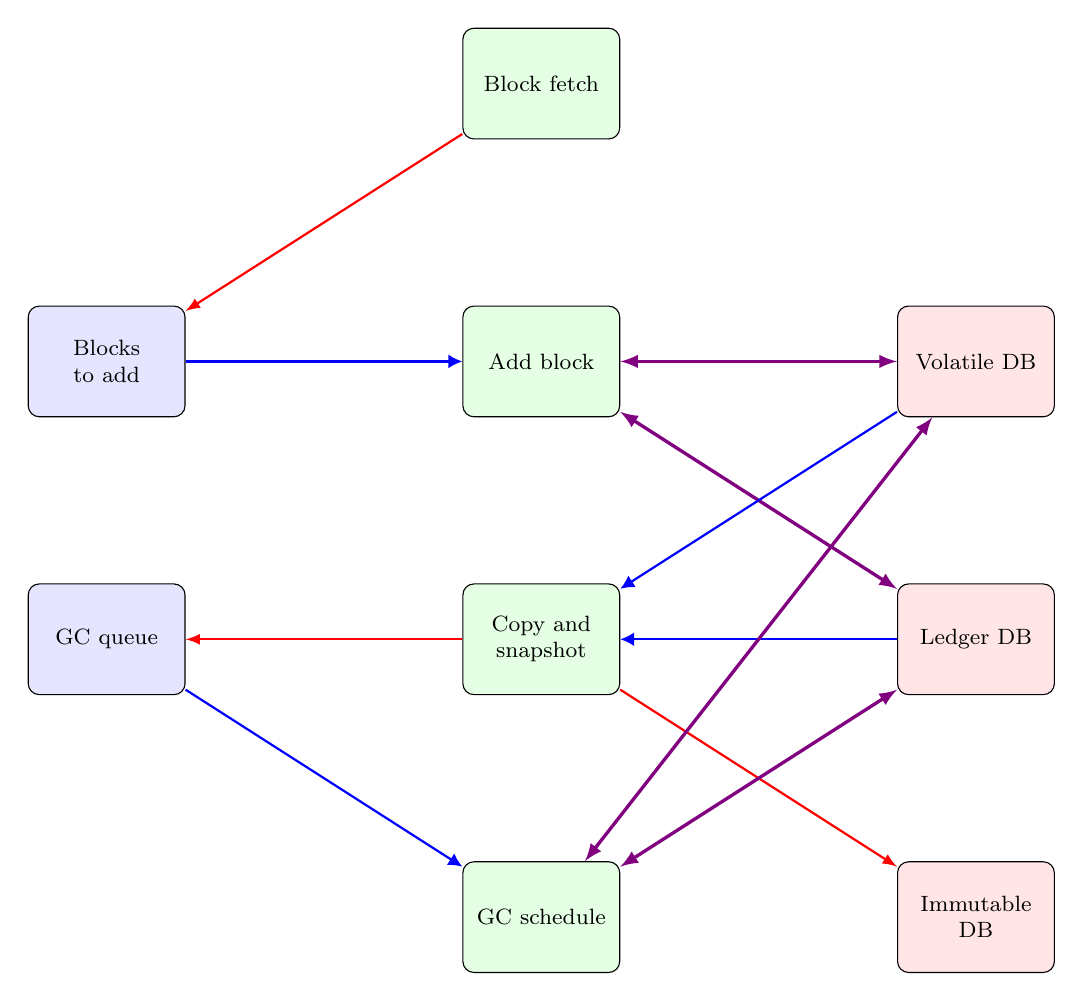
\begin{tikzpicture}[ align             = center
                     , text width        = 5em
                     , font              = \footnotesize
                     , every node/.style = { rectangle
                                           , rounded corners
                                           , draw           = black
                                           , align          = center
                                           , minimum height = 4em
                                         }
                     % Use latex style arrows
                     , >={Latex[width=0.5em, length=0.5em]}
                     , node distance = 6em and 10em
                     ]

  %%
  %% Node types
  %%
  \tikzset{ process/.style={fill=green!10}
          , db/.style={fill=red!10}
          , queue/.style={fill=blue!10}
          , dummy/.style={draw=none}
          }

  %%
  %% Arrow types
  %%
  \tikzset{ read/.style={->, blue, thick}
          , write/.style={-latex, red, thick}
          , rw/.style={latex-latex, violet, very thick}
          }

  %%
  %% Nodes
  %%
  \node (abr) [process                ] {Add block};
  \node (bf)  [process, above = of abr] {Block fetch};
  \node (csr) [process, below = of abr] {Copy and snapshot};
  \node (gcr) [process, below = of csr] {GC schedule};

  \node (vdb) [db, right = of abr] {Volatile DB};
  \node (ldb) [db, below = of vdb] {Ledger DB};
  \node (idb) [db, below = of ldb] {Immutable DB};

  \node (gcq) [queue, above left = of gcr] {GC queue};

  \node (bta) [queue, above = of gcq] {Blocks to add};

  %%
  %% Relationships between nodes
  %%
  \path[write] (bf) edge (bta);

  %%% Add block runner
  \path[read] (bta) edge (abr);
  \path[rw] (vdb.west) edge (abr.east);
  \path[rw] (ldb) edge (abr);

  %%% Copy an snapshot runner
  \path[read] (ldb) edge (csr);
  \path[read] (vdb) edge (csr); % TODO: this is based on the comments only. We need to confirm with the code.
  \path[write] (csr) edge (idb); % TODO: this is based on the comments only. We need to confirm with the code.

  %%% GC schedule
  \path[rw] (gcr) edge (ldb);
  \path[rw] (gcr) edge (vdb);

  %%% Queue connection
  \path[write] (csr) edge (gcq);
  \path[read] (gcq) edge (gcr);

  \end{tikzpicture}
  \caption{Storage layer background processes}
  \label{fig:storage-layer-background-processes}
\end{figure}


\end{document}
%%% Local Variables:
%%% mode: latex
%%% TeX-master: t
%%% End:
